%%%%%%%%%%%%%%%%%%%%%%%%%%%%%%%%%%%%%%%%%%%%%%%%%%%%%%%%%%%%%%%%%%%%%%
%     File: ExtendedAbstract_backg.tex                               %
%     Tex Master: ExtendedAbstract.tex                               %
%                                                                    %
%     Author: Andre Calado Marta                                     %
%     Last modified : 27 Dez 2011                                    %
%%%%%%%%%%%%%%%%%%%%%%%%%%%%%%%%%%%%%%%%%%%%%%%%%%%%%%%%%%%%%%%%%%%%%%
% A Theory section should extend, not repeat, the background to the
% article already dealt with in the Introduction and lay the
% foundation for further work.
%%%%%%%%%%%%%%%%%%%%%%%%%%%%%%%%%%%%%%%%%%%%%%%%%%%%%%%%%%%%%%%%%%%%%%

\section{Background}
\label{sec:backg}

In this section we summarize the main aspects of the three most important parts of this work: the tight-binding model used to describe TMD nanoribbons, and its extension to the interacting case via on-site intra-orbital interactions; the mean field theory of this model, and the iterative solution of the corresponding self-consistent equation; the simulation of the model using Determinant Quantum Monte Carlo.

\subsection{Minimal 3-band tight-binding model}

Here, we present a minimal model describing the low energy physics of group 6 TMD monolayers \cite{liu_three-band_2013}.
To obtain this tight-binding model, one uses the symmetries of the monolayer, and the fact that at low energies, both band edges have major contributions from $d_{z^2}$, $d_{xy}$, and $d_{x^2 - y^2}$ orbitals of M-atoms and the $p$-orbitals of the X-atoms (which contribute very little at the band edges).
This is illustrated for $\text{Mo}\text{S}_2$ in Fig.(\ref{fig:nanoribbons_energiesTMDs}).
Near the Fermi energy, the $\text{Mo}$ $d$-orbitals are clearly more populated at the $K$ point (circled in orange), hence these atomic orbitals contribute more to the Bloch states near that point.
\begin{figure}[H]
\centering
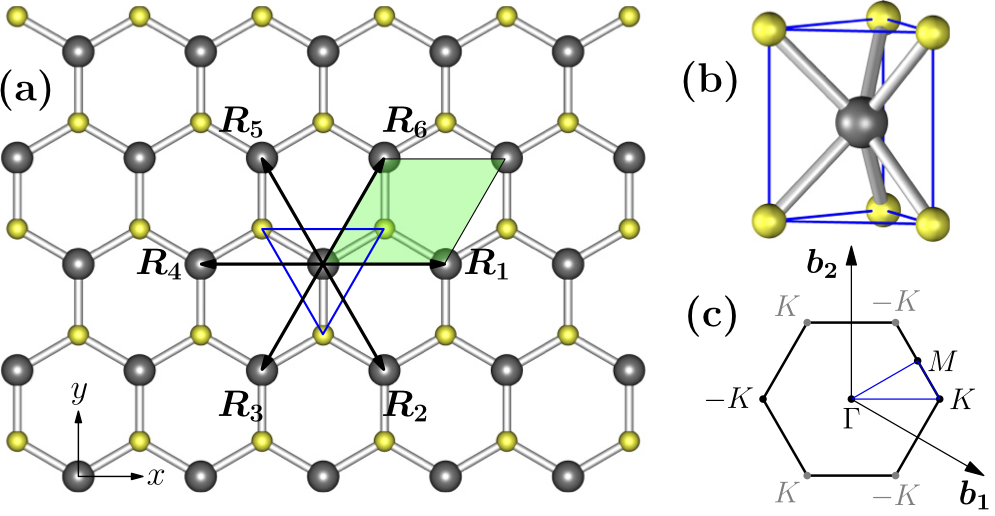
\includegraphics[scale = 0.2]{images/tmd2.png}
 \caption{(a) The 2H phase of a  TMD monolayer may be viewed simply as a $M-X$ honeycomb lattice. Here we represent the six nearest neighbors of a point on the $M$ triangular lattice by the real space vectors $\bm R_{i = 1,2,..., 6}$.
(b) Unit cell of the trigonal prismatic (2H) phase of a TMD monolayer.
(c) High symmetry points $\Gamma, M, K$ of the first Brillouin zone ($\bm b_{1,2}$ are the reciprocal basis vectors).\label{fig:tmdHex}}
\end{figure}
The existence of mirror symmetry through the $x-y$ plane (see Fig.(\ref{fig:tmdHex})) imposes that no hybridization can occur between the sets of orbitals $\{d_{z^2}, d_{xy}, d_{x^2 - y^2} \}$ and $\{d_{xz}, d_{yz} \}$ ($d_{yz}$ and $d_{xz}$ orbitals are not symmetric under reflection upon the $x-y$ plane).
At low energies, the former are known to be the most relevant for the band structure of TMDs (see Fig.(\ref{fig:nanoribbons_energiesTMDs})).
These considerations motivate us to construct a three-band tight-binding model.
\begin{figure}[H]
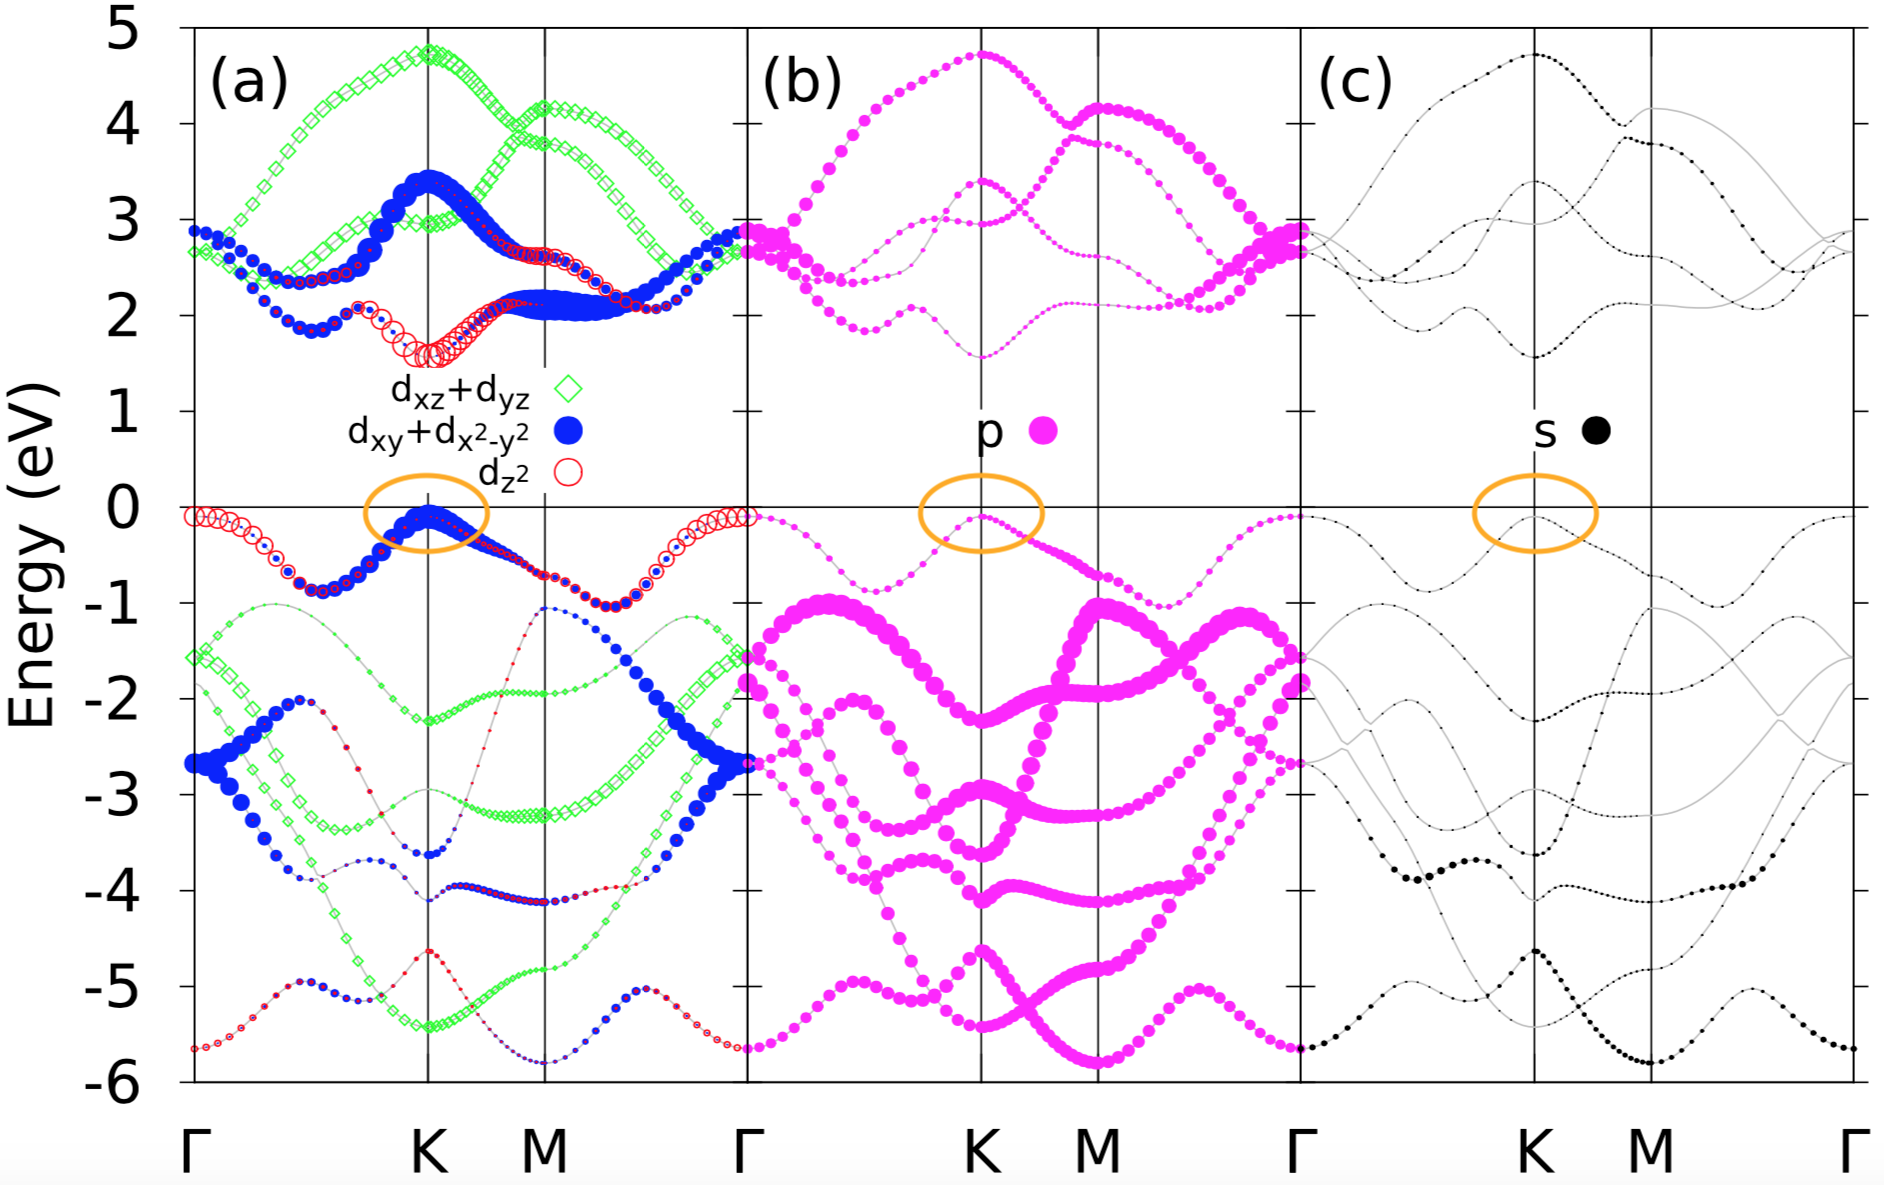
\includegraphics[scale = 0.2]{images/energiesTMDs}
 \caption{Orbital projected band structures for monolayer $\text{Mo}\text{S}_2$ obtained from first principles.
The Fermi energy is set to 0, and the symbol size is proportional to the population of the state.
The panels represent the contributions from: (a) $\text{Mo}$ $d$-orbitals; (b) All $p$-orbitals, dominated by $\text{S}$ atoms; (c) All $s$-orbitals. \label{fig:nanoribbons_energiesTMDs}}
\end{figure}
Moreover, the remaining point-symmetry operations impose a constraint on the number of independent hopping parameters.
By fitting to first principles results obtained from density functional theory %(using both the local-density and the generalized gradient approximations - LDA and GCA) 
for the materials' energy bands, the hopping parameters can be obtained.
The strategy that is chosen to do the fit in \cite{liu_three-band_2013} is to fit the band energies at the high-symmetry $\bm k$-points $\Gamma$, $K$, and $M$, and the energies of the valence and conduction bands near $K$ by least-squares.
This procedure leads to a non-uniform nearest neighbor (NN) hopping matrix on the M-atom triangular lattice.
Note that since the argument is purely based on symmetry, in general, the $d-d$ hoppings include both direct $d-d$ interactions of M atoms, and indirect ones, mediated by $X-p$ orbitals.
These M-M hoppings suffice to describe the band-edge properties near the $\pm K$ valleys.
By including third nearest neighbor hoppings, one can reproduce the energy dispersion in  the entire first Brillouin zone.
We consider a \say{spinless} model.
Let the greek indices represent orbital space, except for $\sigma$, meaning spin.
Then, the  tight-binding Hamiltonian reads
\begin{equation}
\mathcal{H} = \sum_{i, j, \sigma} \sum_{\alpha, \beta} c_{i,\alpha}^\dagger t_{\alpha \beta}^\sigma ( \bm R_i - \bm R_j ) c_{j, \beta} , t_{\alpha \beta}^\downarrow ( \bm R ) = t_{\alpha \beta}^\uparrow ( \bm R )
\end{equation}
where we consider the basis set $\{ \left| \alpha \right\rangle \}_{\alpha = 1}^3 = \{ (d_{z^2}) , (d_{x y}, d_{ x^2 - y^2 }) \} $.
Let 
\begin{equation*}
\begin{split}
\varepsilon_1 &= t_{11}^{11} ( \bm 0 ) \quad \varepsilon_2 = t_{22}^{11} ( \bm 0 ) = t_{22}^{22} ( \bm 0 ) \\
t_0 &= t_{11}^{11} ( \bm R_1 ) \quad t_1 = t_{11}^{12} ( \bm R_1 ) \quad t_2 = t_{12}^{12} ( \bm R_1 ) \\
t_{11} &= t_{11}^{22} ( \bm R_1 ) \quad t_{12} = t_{12}^{22} ( \bm R_1 ) \quad t_{22} = t_{22}^{22} ( \bm R_1 )
\end{split}
\end{equation*}

The on-site energies $\varepsilon_j$ corresponding to the atomic orbitals $\left| \phi_\mu^j \right\rangle$ appear through a diagonal hopping matrix in orbital space $\bm t ( \bm 0 ) \equiv \bm t^0 = \text{diag} ( \varepsilon_1, \varepsilon_2, \varepsilon_2 )$, while the NN hoppings are (see Fig.(\ref{fig:tmdHex}))
\begin{equation}
\bm t (\bm R_{1, 4}) \equiv \bm t^{1, 4} =
\begin{pmatrix}
t_0 & \pm t_1 & t_2 \\
\mp t_1 & t_{11} & \pm t_{12} \\
t_2 & \mp t_{12} & t_{22} \\
\end{pmatrix}
\end{equation}
\begin{strip}
\begin{equation}
\bm t (\bm R_{2,5\,(3,6)})  \equiv \bm t^{2, 5 (3, 6)}  =
\begin{pmatrix}
t_0 & \Pm \bigg( \pm \frac{1}{2} t_1 - \frac{\sqrt{3}}{2} t_2 \bigg) & \mp \frac{\sqrt{3}}{2} t_1 - \frac{1}{2} t_2 \\
\Pm \bigg( \mp \frac{1}{2} t_1 - \frac{\sqrt{3}}{2} t_2 \bigg) & \frac{1}{4} ( t_{11} + 3 t_{22} ) & \Pm \bigg( \frac{\sqrt{3}}{4} ( t_{22} - t_{11} ) \mp t_{12} \bigg) \\
\pm \frac{\sqrt{3}}{2} t_1 - \frac{1}{2} t_2 & \Pm \bigg( \frac{\sqrt{3}}{4} ( t_{22} - t_{11} ) \pm t_{12} \bigg) & \frac{1}{4} ( 3 t_{11} + t_{22} )
\end{pmatrix}
\end{equation}
\end{strip}

The model we consider is obtained by adding intra-orbital on-site interactions to this model.
Let $\bm K = \bm K_{\text{site}} \otimes \bm K_{\text{orb}}$ be the hopping matrix whose elements are the hoppings between the orbital $\alpha$ of site $i$ and the orbital $\beta$ of site $j$.
Then, the intra-orbital Hubbard-like model corresponding to this minimal 3-band tight-binding model reads
\begin{strip}
\begin{equation}\label{eq:tmdHam}
\mathcal{H} = \overbrace{- \sum_{\substack{i, j \\ \alpha, \beta, \sigma}} K_{(i\alpha),(j\beta )} \bigg( c_{i,\alpha, \sigma}^\dagger c_{j,\beta, \sigma} + c_{j,\beta , \sigma}^\dagger c_{i,\alpha, \sigma} \bigg)}^{\mathcal{H}_K} + \underbrace{\frac{U}{2} \sum_{\substack{i, \alpha \\ \sigma \neq \sigma'} } n_{i\alpha, \sigma} n_{i\alpha, \sigma'}}_{\mathcal{H}_V}
\end{equation}
\end{strip}

\subsection{Self-consistent solution in the GCE}\label{subsec:selfconsistent}

Here, we show how to solve the mean field Hamiltonian in an iterative, self-consistent manner.
\begin{strip}
\begin{equation}
\mathcal{H}_{\text{MF}} = \mathcal{H}_\uparrow + \mathcal{H}_\downarrow + \mathcal{C} , \,\, \mathcal{H}_\sigma = - t \sum_{\left\langle i, j \right\rangle} \bigg( c_{i,\sigma}^\dagger c_{j,\sigma} + c_{j,\sigma}^\dagger c_{i,\sigma} \bigg) + U \sum_i n_{i,\sigma} \left\langle n_{i,-\sigma} \right\rangle , \,\, \mathcal{C} = - U \sum_i \left\langle n_{i,\uparrow} \right\rangle \left\langle n_{i,\downarrow} \right\rangle
\end{equation}
\end{strip}

We seek the most energetically favorable self-consistent solution iteratively\footnote{One must pay attention so as not to get stuck in metastable states.}: the up and down-spin electron densities are updated successively until convergence occurs.

Since the interacting problem is turned into a single particle problem, the solution basically consists of diagonalizing two $N \times N$ matrices, where $N$ is the size of the system.
By varying the $2N$ mean field parameters, which are essentially the average local densities $\left\langle n_{i,\sigma} \right\rangle$, we can find the ground state, or other excited states, at the mean field level.
The mean field approach has several advantages: the Hilbert space is reduced from exponential to linear in the system size, which allows the study of relatively large systems; we can do the computation in real space; we can arbitrarily change the system geometry (introducing OBC, defects, nonuniform hoppings); the model is flexible: tight-binding, and interaction terms are easily added to the Hamiltonian.
However, $SU(2)$ symmetry is broken, and electron correlations are neglected.
Only long range order is captured and its stability is often overestimated.
While the mean field solution approaches the exact solution at weak coupling $U$, it can give only qualitative behavior at best, when $U$ increases significantly.

The iterative method starts with the initialization of the mean field parameters.
This initial condition cannot be completely arbitrary because it affects convergence.
Typical choices are the random initial condition or the paramagnetic state.
Then, we repeat the following steps until convergence.

First, we diagonalize $\mathcal{H}_\sigma$, obtaining the one-particle spectrum $\varepsilon_{\alpha, \sigma}$ and the corresponding eigenvectors.
\begin{equation}
\mathcal{H}_{\text{MF}} = \sum_{\alpha, \sigma} \varepsilon_{\alpha, \sigma} d_{\alpha, \sigma}^\dagger d_{\alpha, \sigma} + \mathcal{C} , \,\, d_{\alpha, \sigma} = \sum_i Q_{\alpha i, \sigma}^\star c_{i,\sigma}
\end{equation}

Given a number of electrons per unit cell, $n_e$, compute the chemical potential corresponding to that filling implicitly through $ \frac{1}{N} \sum_{\alpha, \sigma} (  e^{\beta ( \varepsilon_{\alpha, \sigma} - \mu ) } +1 )^{-1} = n_e$ (we use the bissection method).

Recompute mean field parameters, and check for convergence: at iteration $I$, $\left\langle n_{i,\sigma} \right\rangle_I \approx \left\langle n_{i,\sigma} \right\rangle_{I - 1}$.
\begin{equation}\label{eq:selfConsistent}
\left\langle n_{i,\sigma} \right\rangle = \sum_\alpha | Q_{\alpha i, \sigma} |^2 ( 1 + e^ { \beta ( \varepsilon_{\alpha, \sigma} - \mu )} )^{-1}
\end{equation}

Now, we discuss how to circumvent the convergence issues that may arise when applying the self-consistent procedure.
First, there are many possible initial conditions, most notably: the random one, which is the most unbiased, but may be slow or not converge at all; the paramagnetic state $\left\langle n_{i,\sigma} \right\rangle = \text{const.}$, which, when combined with the annealing method we shall describe below, emulates the random initial condition; a specific state, such as the antiferromagnetic one, which is a biased choice, which limits the accessible part of parameter space, and potentially gives a misleading mean field solution, but can have good convergence properties.
In some cases, the symmetry of the system dramatically slows down convergence.
By starting the procedure at a higher temperature than the desired one, we can improve convergence.
The temperature is then gradually lowered until the desired one is achieved, and this procedure is applied at that temperature.
There are a lot of possible annealing schemes, namely keeping $\beta$ fixed for some iterations and then adjusting it to the desired $\beta = \beta_0$, or smoothly reducing $\beta$ until it reaches $\beta_0$.
A common convergence issue is the oscillation between two configurations $\left\langle n_{i,\sigma}\right\rangle_I \leftrightarrow \left\langle n_{i,\sigma}\right\rangle_{I+1}$.
This is solved by averaging the values obtained at the current and previous iterations: $\left\langle n_{i,\sigma}\right\rangle_{I+1} \leftarrow \frac{1}{2} \left\langle n_{i,\sigma}\right\rangle_I + \frac{1}{2} \left\langle n_{i,\sigma}\right\rangle_{I+1}$
The weights attributed to each configuration can be also be different, or even vary with the iteration: $\left\langle n_{i,\sigma}\right\rangle_{I+1} \leftarrow P(I) \left\langle n_{i,\sigma}\right\rangle_I + (1 - P(I) ) \left\langle n_{i,\sigma}\right\rangle_{I+1}$, if we make sure that $P(I) > \delta$, the latter being the convergence parameter.
Finally, the number of parameters may be reduced.
This is done while taking into account the symmetry of the system.
For example, one may take only the number of sublattices, say 2 for a square lattice with PBC.
This corresponds to the uniform density ansatz $\left\langle n_{i,\sigma} \right\rangle = n_X = \frac{1}{N_X} \sum_{i \in X} \left\langle n_{i,\sigma} \right\rangle$ for all sites in the $X$ sublattice.
If this reduction is not done correctly, we will obtain biased self-consistent solutions that do not necessarily reflect the nature of the solution.

In general, our mean field formulation would involve diagonalizing an $N \times N$ matrix at each step, where $N = N_{\text{orb}} N_x N_y$ is the size of the system times the number of orbitals.
However, since we consider PBCs along the $x$-direction, we can partially diagonalize  the Hamiltonian analytically, reducing the size of the matrix to be diagonalized to $N_{\text{orb}} N_y \times N_{\text{orb}} N_y$, where $N_y$ is the width of the ribbon, i.e. the number of $\text{M}\text{X}_2$ formula units.
Consider the spinless 3-band tight binding model, with unit lattice constant:
\begin{strip}
\begin{equation}
\begin{split}
\mathcal{H}_0 &= \sum_{\substack{m, n \\ \alpha, \beta}} \bigg( c_{m,n, \alpha}^\dagger t_{\alpha\beta}^0 c_{m, n, \beta} + \delta_{0, N_x}  c_{m,n, \alpha}^\dagger t_{\alpha\beta}^1 c_{m+1, n, \beta} + \delta_{-\sqrt{3}/2, (N_y -1)\sqrt{3}/2}  c_{m,n, \alpha}^\dagger t_{\alpha\beta}^4 c_{m-1, n, \beta} \\
& + \delta_{0, N_m} \delta_{-1, (N_y -1)\sqrt{3}/2} c_{m+1/2,n-\sqrt{3}/2, \alpha}^\dagger t_{\alpha\beta}^2 c_{m, n, \beta} + \delta_{-1, (N_y -1)\sqrt{3}/2} c_{m-1/2,n-\sqrt{3}/2, \alpha}^\dagger t_{\alpha\beta}^3 c_{m, n, \beta} \\
& + \delta_{N_y\sqrt{3}/2, 0} c_{m+1/2,n+\sqrt{3}/2, \alpha}^\dagger t_{\alpha\beta}^6 c_{m, n, \beta} + \delta_{-1, N_x -1} \delta_{N_y\sqrt{3}/2, 0} c_{m-1/2,n+\sqrt{3}/2, \alpha}^\dagger t_{\alpha\beta}^5 c_{m, n, \beta} \bigg)
\end{split}
\end{equation}
Fourier transforming along $m$: $c_{m, n, \alpha} = \frac{1}{\sqrt{N_x}}\sum_{k} e^{-i k m } c_{k, n, \alpha} $, with $k = \frac{2\pi}{N_x} \{ -\frac{N_x}{2} + 1, -\frac{N_x}{2}, ..., \frac{N_x}{2} \}$:
\begin{equation}
\begin{split}
\mathcal{H}_0 &= \sum_{ \substack{k, y \\ \alpha, \beta} } \bigg( c_{k, y, \alpha}^\dagger (t_{\alpha \beta}^0  + e^{ik} t_{\alpha \beta}^1 + e^{-ik} t_{\alpha \beta}^4 )  c_{k, y, \beta} + \delta_{-1, N_y -1} c_{k, y - 1, \alpha}^\dagger ( e^{ik/2} t_{\alpha \beta}^2 + e^{-ik/2} t_{\alpha \beta}^3 ) c_{k, y, \beta} \\
& + \delta_{N_y, 0} c_{k, y, \alpha}^\dagger ( e^{ik/2} t_{\alpha \beta}^6 + e^{-ik/2} t_{\alpha \beta}^5 ) c_{k, y+1, \beta} \bigg) , \,\, \text{with} \, y \, \text{defined as in Fig.(4.1)}
\end{split}
\end{equation}
leading to a tridiagonal block $3 N_y \times 3 N_y$ hopping matrix $\bm H (k)$ with three different types of matrix elements: $\bm h_1 = \bm H_{y,y}$, $\bm h_2 = \bm H_{y,y-1}$, $\bm h_2^\dagger = \bm H_{y, y+1}$.
\begin{equation}
[ H_{(\alpha y) (\beta y')} (k) ] = 
\begin{pmatrix}
\bm h_1 & \bm h_2^\dagger & & & \\
\bm h_2 & \bm h_1 & \bm h_2^\dagger & & \\
& \bm h_2 & \bm h_1 & \ddots & \\
& & \ddots & \ddots & \bm h_2^\dagger \\
& & & \bm h_2 & \bm h_1
\end{pmatrix}, \, 
\bm h_1 = 
\begin{pmatrix}
\varepsilon_1 + 2 t_0 \cos k & 2 i t_1 \sin k & 2 t_2 \cos k \\
-2 i t_1 \sin k & \varepsilon_2 + 2 t_{11} \cos k & 2 i t_{12} \sin k \\
2 t_2 \cos k& -2 i t_{12} \sin k & \varepsilon_2 + 2 t_{22} \cos k \\
\end{pmatrix}
\end{equation}
\begin{equation*}
\bm h_2 =
\begin{pmatrix}
2 t_0 \cos ( k / 2 ) & i \sin ( k / 2 ) \bigg( t_1 - \sqrt{3} t_2 \bigg) & - \cos (k /2 ) \bigg( \sqrt{3} t_1 + t_2 \bigg) \\
-i \sin ( k / 2 ) \bigg(t_1 + \sqrt{3} t_2 \bigg) & \frac{1}{2} \cos (k / 2) \bigg( t_{11} + 3 t_{22} \bigg) & -i \sin (k / 2) \bigg( \frac{\sqrt{3}}{2} (t_{11} -  t_{22} ) + 2 t_{12} \bigg) \\
\cos ( k / 2) \bigg( \sqrt{3} t_1 - t_2 \bigg) & -i \sin (k / 2) \bigg( \frac{\sqrt{3}}{2} ( t_{11} - t_{22} ) - 2 t_{12} \bigg) & \frac{1}{2} \cos (k / 2) \bigg( 3 t_{11	} + t_{22} \bigg)
\end{pmatrix}
\end{equation*}
\end{strip}
By applying our mean field approach to solve the 3-band model with Hubbard-type interactions, we obtain solutions that are independent of $x$ (the longitudinal coordinate on the ribbon), which motivates us to reduce the number of MF parameters by choosing a translationally invariant ansatz.
This is equivalent to taking $\left\langle n_{x, y,\alpha, \sigma}\right\rangle = \left\langle n_{y,\alpha, \sigma}\right\rangle  \forall x$ ($6 N_y$ parameters).
By reducing the number of parameters, convergence is facilitated, which allows us to evaluate whether the solution of Fig.(\ref{fig:nanoGraphVsTMD}) is robust, i.e. whether it corresponds to a metastable or not.
The mean field form of the interaction term with the reduced number of parameters changes, implying that the self-consistent relation of Eq.(\ref{eq:selfConsistent}) from which the local densities are computed changes as well.
\begin{strip}
\begin{equation}
\mathcal{H}_{\text{MF}} = \mathcal{H}_0 + \mathcal{H}_1 + \mathcal{C} , \,\text{where} \,\, \mathcal{H}_1 = U \sum_{m, n, \alpha}  \sum_\sigma n_{\substack{m, \sigma \\ n, \alpha}} \big\langle n_{\substack{m, -\sigma \\ n, \alpha}} \big\rangle  , \,\, \mathcal{C} = -U  \sum_{m, n, \alpha} \big\langle n_{\substack{m, \uparrow \\ n, \alpha}} \big\rangle \big\langle n_{\substack{m, \downarrow \\ n, \alpha}} \big\rangle
\end{equation}
\begin{equation}
\begin{split}
\mathcal{H}_1 + \mathcal{C} &= \frac{U}{N_x^{\,2}} \sum_{\substack{n \alpha \\ k_1 k_2 \\ k_3 k_4}} \underbrace{\sum_m e^{i [ (k_1 + k_3) - (k_2 + k_4) ] m}}_{N_x \delta_{k_4, k_1 + k_3 - k_2}} \bigg( \sum_\sigma c_{\substack{k_1, \sigma \\ n, \alpha}}^\dagger c_{\substack{k_2, \sigma \\ n, \alpha}} \underbrace{\big\langle c_{\substack{k_3, -\sigma\\ n, \alpha}}^\dagger c_{\substack{k_4, -\sigma \\ n, \alpha}} \big\rangle}_{\delta_{k_3, k_4} \big\langle n_{\substack{k_3,-\sigma \\ n, \alpha}} \big\rangle} - \underbrace{\big\langle c_{\substack{k_1, \uparrow \\ n, \alpha}}^\dagger c_{\substack{k_2  \uparrow \\n, \alpha}} \big\rangle}_{\delta_{k_1, k_2} \big\langle n_{\substack{k_2,\uparrow \\ n, \alpha}} \big\rangle} \underbrace{\big\langle c_{\substack{k_3, \downarrow \\ n, \alpha}}^\dagger c_{\substack{k_4, \downarrow \\ n, \alpha}} \big\rangle}_{\delta_{k_3, k_4} \big\langle n_{\substack{k_3,\downarrow \\ n, \alpha}} \big\rangle}  \bigg) \\
&= \frac{U}{N_x} \sum_{\substack{n \alpha \\ k_2 k_3}} \bigg( \sum_\sigma n_{\substack{k_2, \sigma \\ n, \alpha}} \big\langle n_{\substack{k_3, -\sigma \\ n, \alpha}} \big\rangle - \big\langle n_{\substack{k_2, \uparrow \\ n, \alpha}} \big\rangle \big\langle n_{\substack{k_3, \downarrow \\ n, \alpha}} \big\rangle \bigg) \equiv
U \sum_{k, \mu} \bigg( \sum_\sigma n_{k,\mu, \sigma} \big\langle n_{\mu, -\sigma} \big\rangle - \big\langle n_{\mu, \uparrow} \big\rangle \big\langle n_{\mu, \downarrow} \big\rangle \bigg)
\end{split}
\end{equation}
\end{strip}
where we collapsed the indexes $(n, \alpha)$ into a single index $\mu$.
The self consistent relation allowing us to compute the new MF parameters at each step emerges by diagonalizing $\mathcal{H}_1$ in the $\mu$-subspace:
\begin{equation}
\begin{split}
&\big\langle n_{\mu, \sigma} \big\rangle = \frac{1}{N_x}\sum_{q, \nu} | Q_{q \sigma \mu, \nu} |^2 \rho ( \varepsilon_{q \nu \sigma} ), \\ &\text{where} \,\, d_{q, \sigma, \nu} = \sum_\nu Q_{q \sigma \mu, \nu}^\star c_{q ,\sigma, \mu} , \\ 
& \text{and} \,\, \mathcal{H}_{\text{MF}} = \sum_{q, \nu, \sigma} \varepsilon_{q, \nu, \sigma} d_{q, \nu, \sigma}^\dagger d_{q, \nu, \sigma} + \mathcal{C}
\end{split}
\end{equation}

\subsection{Auxiliary field Quantum Monte Carlo}
\label{sec:afqmc}
This is based on introducing an additional lattice field that mediates the electron-electron interaction.
The interacting problem then becomes a problem of independent fermions coupled to this external field, and the fermionic part of the partition function can be traced out explicitly, leaving the contribution of a \emph{discrete}\footnote{The introduced field is discrete (and \emph{binary}) because each fermionic state can only have occupations $n = 0, 1$. Although, there is a finite number of field configurations, the number grows exponentially with the number of sites on the lattice.} classical field, $\bm h$.
This contribution can be evaluated numerically by employing importance sampling over the field configurations.
Auxiliary field QMC relies on a mapping to a so called \say{classical} system (in quotes because there may be no actual classical analogue):
\begin{equation}\label{eq:Zsign}
Z = \Tr [ e^{-\beta \mathcal{H} } ] = \sum_{\{ \bm h\} } \sum_{\text{fermionic}} e^{-S} = \sum_c p_c ,
\end{equation}
but some of the \say{probabilities} $p_c$ can actually be negative due to the antisymmetry of the many-electron wavefunction under electron exchange.
Here, $S$ is a fermion-field action that we shall write out explicitly later.
For a fixed configuration of the $\bm h$ field, we sum over the fermionic part exactly to obtain the weight of each configuration $p_c$.
The sum over $\bm h$ is carried out stochastically.
The negative weight problem can be circumvented when computing the average of an observable $A$:
\begin{equation}\label{eq:signSampling}
\begin{split}
\left\langle A \right\rangle &= \frac{\sum_c A ( c ) p ( c )}{\sum_c p ( c ) } \\ &= \frac{\sum_c A ( c )|  p ( c ) | \text{sign}[p(c)] / \sum_c | p ( c ) | }{\sum_c  |  p ( c ) | \text{sign}[p(c)] /  \sum_c | p ( c ) |} \equiv \frac{\left\langle A s \right\rangle_{|p|}}{\left\langle s \right\rangle_{|p|}} ,
\end{split}
\end{equation}
where $s(c) = \text{sign} [ p ( c ) ]$, and $| p ( c ) | $ corresponds to an auxiliary bosonic system (also coupled to the classical field) corresponding to the original fermionic system, and for which there is no sign problem.

The relative error $\Delta s / \left\langle s \right\rangle$ increases exponentially with the number of particles, with inverse temperature, and possibly with other parameters of the specific model to be studied \cite{troyer_computational_2005, hou_numerical_2009}.
To see this, we start by noting that the average sign is the ratio between the partition functions of the fermionic ($Z = \sum_c p(c)$) and bosonic systems ($Z' = \sum_c | p ( c ) |$).
In terms of the difference in free energy densities, $\left\langle s \right\rangle = Z / Z' = e^{-\beta N_p \Delta f}$, implying that for $M$ samples, the error of the denominator of Eq. (\ref{eq:signSampling}) becomes
\begin{equation}
\frac{\Delta s}{\left\langle s \right\rangle} = \frac{\sqrt{(\left\langle s^2 \right\rangle - \left\langle s \right\rangle^2 )/ M }}{\left\langle s \right\rangle} = \frac{ \sqrt{ 1 - \left\langle s \right\rangle^2}  }{\sqrt{M} \left\langle s \right\rangle} \propto \frac{e^{\beta N_p \Delta f}}{\sqrt{M}} ,
\end{equation}
and similarly for the numerator of Eq. (\ref{eq:signSampling}).

Mean field theory may be formulated by applying the Hubbard Stratonovich (HS)  transformation to transform an interacting problem into a one-body problem, and then apply the saddle-point approximation to solve the resulting integrals.
In the GCE (where we make $\mathcal{H} \mapsto \mathcal{H} - \mu \mathcal{N}$, $\mathcal{N}$ being the total particle number), the grand-partition function may be written in terms of a functional integral over a space-time dependent field of the exponential of a one-body action
\begin{equation}
Z = \Tr [ e^{-\beta \mathcal{H} } ] = \int \mathcal{D}\bm h \, e^{-S(\bm h) }  \equiv \Tr_{\bm h} [ e^{-S(\bm h)} ],
\end{equation}
which may be computed by Monte Carlo sampling.
In mean field, we approximate the integral by replacing the functional integral by a constant times the exponential of the action - evaluated at the field $\bm h^\star$, for which the action has a minimum: $\partial_{\bm h} S( \bm h ) |_{\bm h = \bm h^\star} = 0$, and $\partial_{\bm h}^2 S( \bm h ) |_{\bm h = \bm h^\star} > 0$.
%The integral is evaluated exactly in the auxiliary field QMC method, which avoids the bias introduced by the specific choice of the HS decoupling.
%The nature of the analytical mean field solution depends on this choice, while the unbiased QMC solution does not, relying on a numerical solution that scales with the cubic volume of the system, and linearly with inverse temperature.
This approach depends on the HS decoupling that was used.
In contrast, with the auxiliary field QMC method, one computes the integral directly.
Although it is more expensive in computing time ($\mathcal{O}(\beta N^3)$ ), it does not rely on any particular choice of the decoupling.
Another obstacle of taking into account all the fluctuations around $\bm h^\star$ is the fermion sign problem.
However, in certain cases, the symmetries of the model (like PHS) may be used to avoid it.
The Trotter-Suzuki decomposition leads to an approximate factorization of $e^{-\beta (\mathcal{H}_K + \mathcal{H}_V )}$ that is used to evaluate the partition function.
Dividing the imaginary time interval $[0, \beta ]$ into $L$ equal sub-intervals of smaller width $\Delta \tau = \beta / L$, one obtains:
\begin{equation}\label{eq:partBreak}
Z =  \Tr \bigg[ \prod_{l=0}^{L-1} e^{-\Delta\tau \mathcal{H} } \bigg] ,
\end{equation}
a form that is more amenable to computation.
Actually, by writing the matrix elements of the projection operator $\mathcal{P}$ as path-integrals (here, time-ordering is implicit \cite{hirsch_discrete_1983}):
\begin{equation}
\begin{split}
&\left\langle \psi | e^{-\beta \mathcal{H} } | \psi' \right\rangle = \sum_{\left| \psi_1 \right\rangle, \left| \psi_2 \right\rangle,..., \left| \psi_{L-1} \right\rangle }  \left\langle \psi | e^{-\Delta \tau \mathcal{H} } | \psi_1 \right\rangle \\
&\left\langle \psi_1 | e^{-\Delta \tau \mathcal{H} } | \psi_2 \right\rangle ... \left\langle \psi_{L - 1} | e^{-\Delta \tau \mathcal{H} } | \psi' \right\rangle ,
\end{split}
\end{equation}
we see that it is the same as the partition function, if the paths are periodic in imaginary time:
\begin{equation}
\begin{split}
Z &= \text{Tr} \big[ e^{-\beta \mathcal{H} } \big] = \sum_{\left| \psi_0 \right\rangle} \left\langle \psi_0 | e^{-\beta \mathcal{H}} | \psi_0 \right\rangle \\
&= \sum_{\{ \left| \psi_l \right\rangle \}} \prod_{l = 0}^{L - 1} \left\langle \psi_{l} | e^{-\Delta \tau \mathcal{H} } | \psi_{l+1} \right\rangle = \Tr \bigg[ \prod_{l=0}^{L-1} e^{-\Delta\tau \mathcal{H}^l } \bigg] ,
\end{split}
\end{equation}
where we have $\left| \psi_L \right\rangle = \left| \psi_0 \right\rangle$. We recover Eq.(\ref{eq:partBreak}) by reorganizing the summations over $\{ \left| \psi_l \right\rangle \}$, and using closure relations in the Hilbert space of each slice.
The \say{Trotter breakup} follows from truncating the inverse of the wellk known Baker-Campbell-Haudsorff formula, and keeping only the first order term in $\Delta \tau$.

The kinetic energy term is quadratic in the fermion operators, and spin-independent, meaning that it be separated into two spin components, independently of the time slice.
\begin{equation}
e^{-\Delta\tau \mathcal{H}_K} = e^{-\Delta\tau \mathcal{H}_{K_\uparrow}} e^{-\Delta\tau \mathcal{H}_{K_\downarrow}} ,
\end{equation}
where $\mathcal{H}_{K_\sigma} = \bm c_\sigma^\dagger (-t_\sigma \bm K_\sigma - \mu_\sigma \bm I )  \bm c_\sigma$.

The potential energy term, however, is quartic.
Fortunately, it is possible to express it in quadratic form by introducing an extra degree of freedom, the so called \emph{Hubbard-Stratonovich (HS) field} $\bm h \equiv (h_{l, i})_{i=0,\, l= 0}^{N-1, \, L - 1}$, in which each element is essentially an Ising spin.
At each slice, the interaction is eliminated by an $N$-dimensional HS field $\widetilde{\bm h}$.
We start by noting that $[ n_{i,\sigma} , n_{j,\sigma'} ] = 0 \,\, \forall i, j, \sigma, \sigma'$, so that in particle-hole symmetric-form\footnote{The particular model in which we are interested does not have particle-hole symmetry (PHS), but the HS transformation is done in PHS-form for convenience when we simulate PHS models.
One simply has to remember that the PHT shifts the chemical potential by $\frac{U}{2}$.}
\begin{equation}\label{eq:Hint}
e^{-\Delta\tau \mathcal{H}_V} = \prod_i e^{-U \Delta\tau (n_{i\uparrow} - 1/2 ) (n_{i\downarrow} - 1/2 )}
\end{equation}
The HS transformation is based on the well known identity 
$
e^{ \frac{a^2}{2}} = \frac{1}{\sqrt{2\pi}} \int_{-\infty}^{\infty} e^{-\frac{z^2}{2}  - za } dz
$ 
$ \forall a > 0$, 
which is also valid if $a$ is an operator $\mathcal{A}$.
Noting that $(n_{i\uparrow} - \frac{1}{2} ) (n_{i\downarrow} - \frac{1}{2} ) = -\frac{1}{2} ( n_{i\uparrow} - n_{i\downarrow} )^2 + \frac{1}{4}$, we can recast the potential energy term as
\begin{equation}\label{eq:gaussianForm}
\begin{split}
&e^{-\Delta\tau \mathcal{H}_V} = \prod_i e^{ \frac{U \Delta \tau}{2} ( n_{i\uparrow} - n_{i\downarrow} )^2 } e^{- \frac{U \Delta \tau}{4}} = \bigg(\frac{\Delta \tau}{\pi} \bigg)^{N/2} \\
& e^{- \frac{N U \Delta \tau}{4}} \int_{-\infty}^\infty \prod_i d \widetilde{h}_i e^{-\Delta \tau [ \widetilde{h}_i^2 + \sqrt{2U} ( n_{i\uparrow} - n_{i\downarrow} ) \widetilde{h}_i ]} ,
\end{split}
\end{equation}
so that in the $\tau \rightarrow 0$ limit, the partition function becomes
\begin{equation}
\begin{split}
Z &\propto \int \mathcal{D} \widetilde{\bm h} ( \tau) e^{-\int_0^\beta d\tau \widetilde{\bm h}^2 ( \tau ) } \\
 &\Tr \bigg[ \mathcal{T}_\tau e^{ -\int_0^\beta d\tau [ \mathcal{H}_K ( \tau ) + \sqrt{2U} ( \bm n_{\uparrow} (\tau) - \bm n_{\downarrow} (\tau ) ) \cdot \widetilde{\bm h}(\tau) ] } \bigg] ,
\end{split}
\end{equation}
representing a system of noninteracting fermions coupled via spin $s^z_i$ to an external fluctuating real field.

The fact that $n_{i,\sigma}$ can only take on two possible values suggests an analogous transformation in which the fluctuating field can only take on two possible values.
An Ising spin will prove sufficient to eliminate the direct electron-electron interaction.
The discrete HS transformation for $U > 0$ allows us to recast Eq.(\ref{eq:Hint}) in terms of the local spin, a non-interacting quadratic term $n_{i\uparrow} - n_{i\downarrow} $ (at each imaginary-time slice, since the operators live on the Hilbert space of that specific slice).
Let $c_U = \frac{1}{2} e^{-\frac{U\Delta \tau}{4}}$ and $\nu = \text{arcosh} ( e^{\frac{U\Delta\tau}{2}})$.
Then, the sought transformation reads
\begin{equation}\label{eq:discreteHS}
e^{-U \Delta\tau (n_{i\uparrow} - 1/2 ) (n_{i\downarrow} - 1/2 )} = c_U \sum_{\widetilde{h}_i = \pm 1} e^{\nu \widetilde{h}_i (n_{i\uparrow} - n_{i\downarrow} )}
\end{equation}

For each imaginary time slice $l$, we may define a HS-field $\widetilde{\bm h_l}$, which specifies $\bm V_l$ and $\mathcal{H}_{V_\sigma}^l$.
The Hamiltonian acquires a \say{ficticious} imaginary-time dependence that enforces (imaginary-)time ordering, and independent Hilbert spaces at each slice.
After some algebra,
\begin{equation}\label{eq:Z_quadratic}
Z  = (c_U)^{NL} \text{Tr}_{\bm h} \Tr \bigg[ \prod_{l=0}^{L-1} \underbrace{\bigg( e^{-\Delta\tau  \mathcal{H}_{K_\uparrow}} e^{\mathcal{H}_{V_\uparrow}^l} \bigg)}_{B_{l, \uparrow}(\widetilde{\bm h_l)}} \underbrace{\bigg( e^{-\Delta\tau  \mathcal{H}_{K_\downarrow}} e^{\mathcal{H}_{V_\downarrow}^l} \bigg)}_{B_{l, \downarrow}(\widetilde{\bm h_l)}} \bigg] ,
\end{equation}
where all operators are now quadratic in the fermion operators:
\begin{equation}
\mathcal{H}_{K_\sigma} = \bm c_\sigma^\dagger ( - t_\sigma \bm K_\sigma -\mu_\sigma \bm I ) \bm c_\sigma \quad \mathcal{H}_{V_\sigma}^l = \sigma \nu \bm c_\sigma^\dagger \bm V_l (\widetilde{\bm h_l}) \bm c_\sigma
\end{equation}
for $\sigma = \pm 1$ and $\bm V_l ( \widetilde{\bm h_l} ) = \text{diag} ( h_{l, 0} , h_{l, 1}, ... , h_{l, N-1} )$.
